\subsubsection{Bayesian Networks}
In this project we will use a modified version of Hidden Markov Models in order to recognize bird calls and possibly other animal sounds. This complicated system starts off with a very fundamental fact of life. ``All models are wrong, but some are useful,'' meaning that getting an exact representation of the real world is impossible. Either some assumptions are incorrect or the way we represent the world leaves out some information. However, while some information will always be left out of a model, it is still possible to construct one that is useful.\par

\begin{center}
  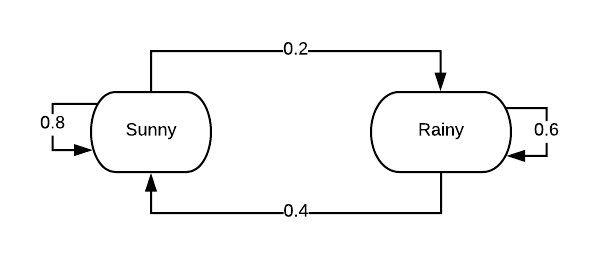
\includegraphics[width=.8\textwidth]{basicmodel}
\end{center}

The models we will be constructing are called probabilistic models. The very bases of these models are that the chance of moving from one state to another can be found out using previous data. After extrapolation, a model of state space and chance of movement between these states can be built. Using the model above as an example, we can see that we have two states: Sunny and Rainy. The chance of either staying in a state or moving from one state to another can be seen by looking at the arrows. The probability of moving is shown as a number from 0 to 1 (0\% to 100\%). While this is not a Bayesian network, it is the very basic idea from which Bayesian networks are built. Using the above model, we can create a conditional probability table (CPT). The corresponding table can be seen below.\par

\begin{center}
	\begin{longtable}{|c|c|c|}
    \hline
		\tablehead{Current}
    & \tablehead{Next}
    & \tablehead{Chance}
    \\ \hline

		Sunny
    & Sunny
    & 0.80
    \\ \hline

		Sunny
    & Rainy
    & 0.20
    \\ \hline

		Rainy
    & Sunny
    & 0.40
    \\ \hline

		Rainy
    & Rainy
    & 0.60
    \\ \hline
	\end{longtable}
\end{center}

Now that we have some idea of what a probabilistic model is, we can apply one of the most useful concepts in Bayesian networks: \textit{conditional independence}. This means that one variable is independent from another variable, depending on given information. The formula for calculating conditional independence is as follows:\par

\begin{equation}
  \textnormal{Independence: }
  P(A|B) = P(A)
\end{equation} \\[\eqnspace]
\begin{equation}
  \textnormal{Conditional Independence: }
  P(A|B,C) = P(A|C)
\end{equation} \\[\eqnspace]

An example of this would be if you have an alarm system. Every time there is a break-in at your house, there is a high chance that the alarm goes off. When the alarm goes off, there is also a chance that your neighbor calls you. Initially with no information, your neighbor calling you will be dependent on whether or not there is a break-in. This changes when you know that the alarm is already ringing. The reasoning for this is that if you already know the alarm is going off, knowing that there is a break in does not give you any more information on the alarm going off. Since the alarm is the only thing that can directly affect your neighbor calling you, then the break-in variable is conditionally unlinked from your neighbor calling you, making the two variables independent.\par
It is possible to map out interactions like this with a Bayesian network, each node being a variable and each arrow connecting two dependent variables. These networks must be acyclic directed graphs. The following figure demonstrates the previous example with added variables: earthquake and one additional neighbor. The alarm is dependent on the earthquake and your other neighbor calling is still dependent only on the alarm.\par

\begin{center}
  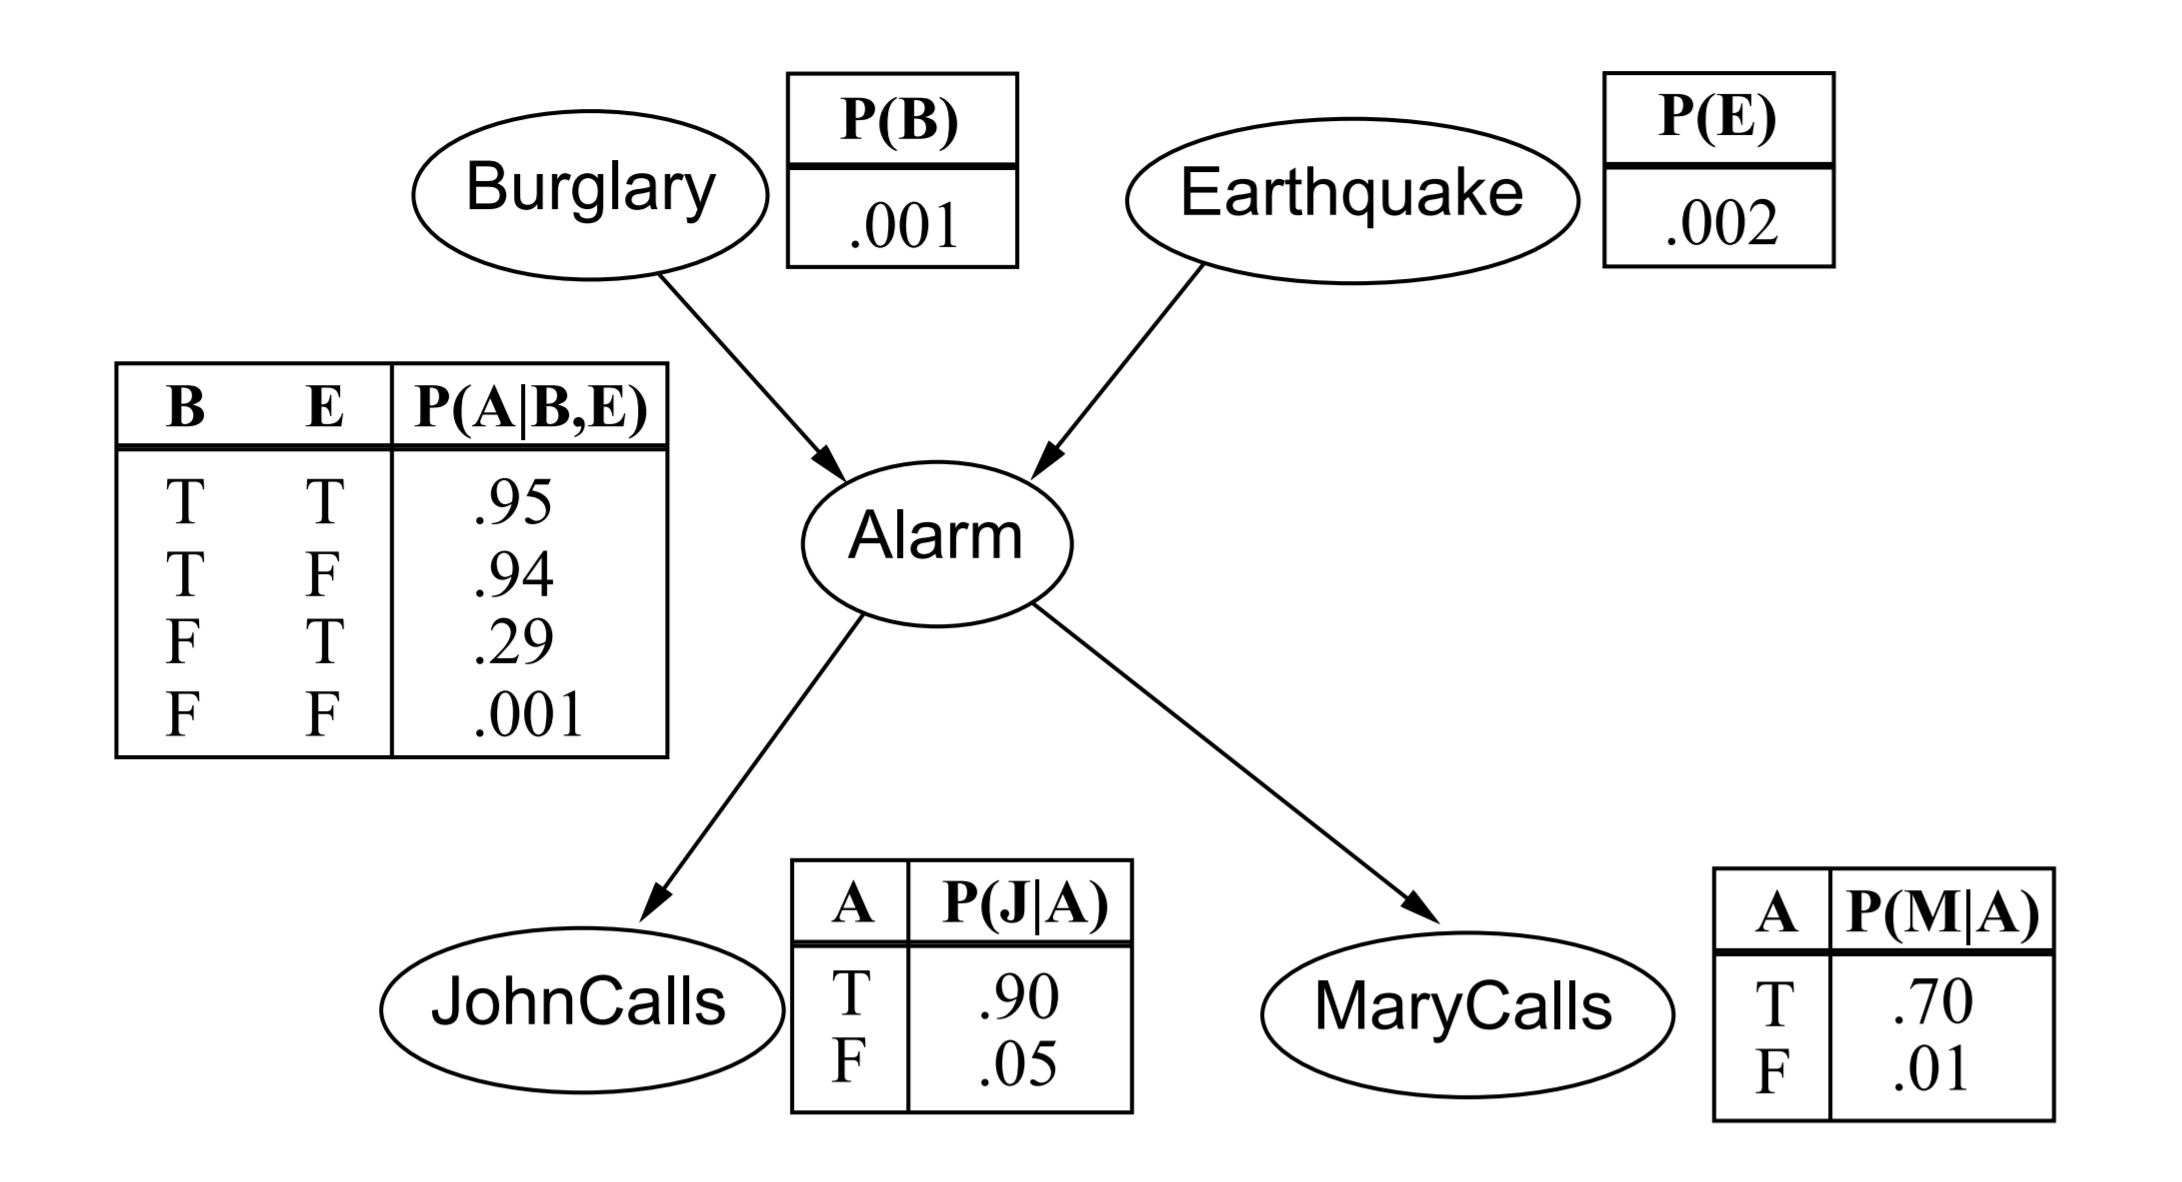
\includegraphics[width=\textwidth]{bayesnet}
\end{center}

With graphs like these, it becomes easier to identify the conditionally independent variables and reduce the size of our corresponding CPT\textquotesingle s. This vastly improves the speed of calculations, since CPT tables grow on a factor of $2^N$ where $N$ is the number of dependent variables. For example, if conditional independence was not used in the figure above, the CPT for JohnCalls would contain 8 (via $2^3$) entries. This is reduced to just 2 entries since Burglary and Earthquake become independent once Alarm is known.
